\documentclass[10pt,a4paper]{article}

\usepackage[utf8]{inputenc}
\usepackage[T1]{fontenc}
\usepackage{amsmath,amssymb,amsfonts}
\usepackage{graphicx}
\usepackage{hyperref}
\usepackage{algorithm}
\usepackage{algpseudocode}
\usepackage{geometry}
\usepackage{cite}

% Page layout
\geometry{margin=1.5cm}

% Title page
\title{\Large\textbf{PixelBytes: Catching Unified Embedding for Multimodal Generation}}
\author{\large Fabien Furfaro}
\date{\large 2024}

\begin{document}

\maketitle

\begin{abstract}
This report presents PixelBytes, an innovative multimodal embedding model designed for the simultaneous generation of text and images pixel by pixel. We introduce the PxByEmbed algorithm as a key component of our architecture, enabling efficient representation of mixed sequences of text and images. Our approach leverages web scraping, image processing, and advanced machine learning techniques to create a unique dataset and training pipeline. We compare the performance of RNN, Transformer, and Mamba models in this task, providing insights into the effectiveness of different architectures for multimodal generation.
\end{abstract}

\begin{figure}[h]
\centering
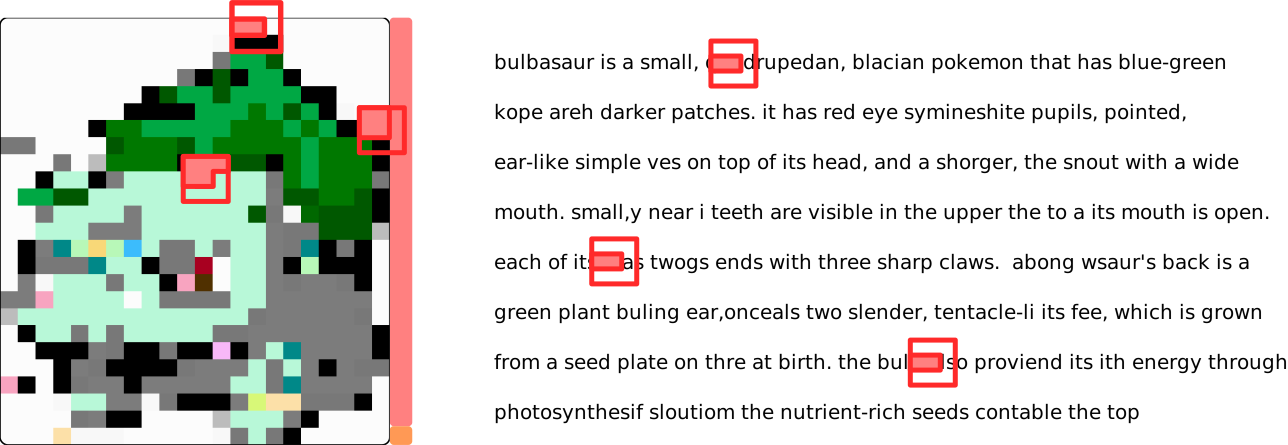
\includegraphics[width=0.8\linewidth]{example_generation.png}
\caption{Example of a generated pixelated Pokémon and its description}
\label{fig:example_generation}
\end{figure}

\section{Introduction}
Multimodal generation, which combines text and images, represents a significant challenge in artificial intelligence. Recent advancements in pixel-by-pixel image generation have shown promising results in creating coherent visual content \cite{parmar2018image}. Plus connu egalmeent les modele de generation de texte comme GPT. Building upon these findings, PixelBytes aims to address the challenge of unified text and image generation by proposing a model capable of producing mixed sequences of text and images in a coherent and unified manner.

Our approach draws inspiration from the state-of-the-art in image transformers, which have demonstrated the ability to generate high-quality images with fine-grained control \cite{parmar2018image}. We also build upon generative sequence models such as GPT, PixelRNN, and PixelCNN. Additionally, we leverage recent developments in bidirectional state space models for time series prediction, which have shown improved performance in capturing long-range dependencies \cite{bimamba}. We also incorporate insights from tokenless selective state space models, which have proven effective in processing sequential data efficiently \cite{mambabyte}.

Notre approche a permis de montrer (...)

\section{Model Architecture}

\subsection{Overview}
PixelBytes integrates several innovative components to achieve its multimodal generation capabilities:
\begin{itemize}
    \item A tokenizer sequence constructor with pixelizable image, and bytes texte
    \item A unified multimodal embedding (PxByEmbed)
\end{itemize}

\subsection{Dataset Construction}

Pour tester notre approche, nous avons besoin d'une base de donnée d'image-captionning. Néanmoins, les bases de données actuelles ne sont pas adapté pour combiner la génération de texte et d'image. Les textes sont souvent trop petit, et une image pixelisé des base de données d'image captionning comme (COCO, Flick) sont difficilement interpretable (les images d'origine sont trop volumineuse). C'est pourquoi, nous avons choisi de construire notre base de donnée à partir des données wiki de Pokemon. Pokemon a l'avantage d'exister depuis plus de 20 ans, lors de l'apparition des jeux video portable, il y a encore des dessins pixelisé ou pixelisable de pokemon. de plus, leur description est une bonne base pour decrire le pokemon. Aujourd'hui, il existe plus de 1000 pokemon, ce qui permet d'avoir une base de donnée minimal pour construire un jeu de données specialisé dans la generation de description et de pixel pokemon.

\subsubsection{Web Scraping from Pokepedia}
We constructed our dataset by scraping miniatures and descriptions from Pokepedia, ensuring a rich and diverse collection of Pokémon data.

Utilisation de beautifull soup. 

\subsubsection{Image Pixelation and Text-Image Balance}
The scraped images were pixelated to create a retro aesthetic. We carefully balanced the dataset to maintain a 2/3 text to 1/3 image ratio, ensuring comprehensive training on both modalities.

Utilisation d'OpenCV et skimage. 

\subsubsection{Image Quantization and Token Creation}
We quantized the pixelated images using a palette inspired by the NES color scheme (55 colors). This process allowed us to create tokens representing different color and position combinations, effectively translating visual information into a format suitable for sequence modeling.

Utilisation d'OpenCV et skimage. (NES palette via le site web des palettes)

Construction des token d'image 

Enregistrement dans le Hub dataset de HuggingFace

\section{Multimodal Embedding Algorithm}

\subsection{PxByEmbed: Multimodal Embedding Algorithm}
At the core of our approach is the PxByEmbed algorithm, which represents mixed sequences of text and images in a unified manner. This algorithm extends classical embedding techniques by incorporating spatial adaptivity, allowing for more effective representation of both textual and visual information.


\begin{algorithm}[h]
\caption{PxByEmbed: Multimodal Embedding Algorithm (k=3)
\newline
\textbf{Input:} $V$: vocabulary size, $D$: embedding dimension
\newline
\textbf{Output:} Embedded representation $\mathbf{E} \in \mathbb{R}^{B \times L \times D}$
\newline
\textbf{Note:} $\mathbf{X}_{emb} \in \mathbb{R}^{B \cdot L \times E_{int} \times k \times k}$, 
$\mathbf{X}_{flat} \in \mathbb{R}^{B \cdot L \times E_{int}k^2}$, 
$\mathbf{X}_{proj} \in \mathbb{R}^{B \cdot L \times D}$
}
\begin{algorithmic}[0]
\State \textbf{Initialize:}
\State $k \gets 3$
\State $E_{int} \gets \max(9, \lfloor D / k^2 \rfloor)$
\State $\mathbf{\alpha} \in \mathbb{R}^{1 \times 1 \times k \times k}$ 
\State $\mathbf{W}_{emb} \in \mathbb{R}^{V \times E_{int}}$ 
\State $\mathbf{W}_{proj} \in \mathbb{R}^{E_{int}k^2 \times D}$ 
\State $\mathbf{W}_{patch} \in \mathbb{R}^{E_{int} \times E_{int} \times k \times k}$ 

\Function{PxByEmbed}{$\mathbf{X} \in \mathbb{Z}^{B \times L \times k \times k}$}
    \State $\mathbf{X}_{emb} \gets \text{Permute}(\text{Embed}(\mathbf{X}, \mathbf{W}_{emb}), [0, 3, 1, 2])$ 
    
    \State $\mathbf{X}_{patch} \gets \text{Conv2D}(\mathbf{X}_{emb}, \mathbf{W}_{patch}, \text{padding}=1)$
    \State $\mathbf{X}_{combined} \gets \sigma(\mathbf{\alpha}) \odot \mathbf{X}_{emb} + (1 - \sigma(\mathbf{\alpha})) \odot \mathbf{X}_{patch}$
    
    \State $\mathbf{X}_{flat} \gets \text{Flatten}(\mathbf{X}_{combined})$ 
    \State $\mathbf{X}_{proj} \gets \mathbf{X}_{flat}\mathbf{W}_{proj}$ 
    \State $\mathbf{E} \gets \text{LayerNorm}(\mathbf{X}_{proj})$
    \State $\mathbf{E} \gets \text{Reshape}(\mathbf{E}, [B, L, D])$
    \State \Return $\mathbf{E}$
\EndFunction
\end{algorithmic}
\end{algorithm}

\subsection{Managing Transitions}
PixelBytes employs newline characters (ASCII 0A) to manage transitions between text and image, ensuring coherence in the generation of mixed sequences.

\section{Model Variants and Training}

\subsection{Model Architectures}
We implemented and compared three different model architectures:
\begin{itemize}
    \item Recurrent Neural Network (RNN)
    \item Transformer
    \item Mamba (State Space Model)
\end{itemize}

\subsection{Training Process}
Training was conducted on dual T4 GPUs from Kaggle, enabling experimentation with these advanced architectures and our large multimodal dataset.

\subsection{Evaluation Metrics}
We employed various metrics to evaluate the performance of our models, including perplexity, BLEU score for text generation, and structural similarity index (SSIM) for image generation.

\section{Results and Discussion}
[This section will be filled with findings and observations from our experiments, including:
- Performance comparison of RNN, Transformer, and Mamba models
- Ablation studies to understand the importance of each component
- Qualitative analysis of generated embeddings and outputs
- Methods and results of measuring similarity in generated sequences]

\section{Conclusion and Future Directions}
This report on PixelBytes opens new avenues in unified multimodal generation. Our findings suggest promising potential for coherent text-image generation. Future work will focus on refining the PxByEmbed algorithm, exploring larger datasets, and investigating applications in creative content generation.

\bibliographystyle{plain}
\bibliography{references}

\end{document}
